\documentclass[12pt, a4paper, oneside]{ctexart}
\usepackage[margin=2cm]{geometry}%要先设置页边距,否则页眉页脚会偏
\usepackage{amsmath, amsthm, amssymb, bm, graphicx, hyperref, mathrsfs,float,xcolor,color}
\usepackage{listings}

% 用来设置附录中代码的样式

\lstset{
    basicstyle          =   \bf \ttfamily,          % 基本代码风格
    keywordstyle        =   \bfseries,   % 关键字风格
    keywordstyle        =   \color{blue},
    stringstyle         =   \color{magenta},
    commentstyle        =   \color{red}\ttfamily,
    language            =    [x86masm]Assembler,
    commentstyle        =   \rmfamily\itshape,  % 注释的风格,斜体
    escapeinside=``, % 英文分号中可写入中文
    stringstyle         =   \ttfamily,  % 字符串风格
    columns=fullflexible,%可以自动换行
    breaklines=true,%在单词边界处换行。
    numbers             =   left,   % 行号的位置在左边
    showspaces          =   false,  % 是否显示空格,显示了有点乱,所以不现实了
    numberstyle         =   \zihao{-5}\ttfamily,    % 行号的样式,小五号,tt等宽字体
    showstringspaces    =   false,
    captionpos          =   t,      % 这段代码的名字所呈现的位置,t指的是top上面
    frame               =   lrtb,   % 显示边框
}
\title{实验十一 \qquad  定时中断}
\author{学号:61822313 \qquad 姓名:钟锦程 \qquad 实验日期:\today}
\date{}
\begin{document}
\maketitle
\section{实验任务和实验结果}
\subsection{基础任务}
\subsubsection{实验任务的具体内容}
本次实验任务为改写定时中断(中断类型号为1CH)的中断服务程序,要求在定时中断服务程序中累计中断次数,每计到50次定时中断就在显示器上显示字符串“SUN”。
主程序:从屏幕左上角到右下角循环显示“太阳”图形,并判断字符串“SUN”的显示次数是否到十次,到十次就结束程序返回DOS。
\subsubsection{调试通过的源程序}
\begin{lstlisting}
    DATA SEGMENT
        STR DB 'SUN',0DH,0AH,'$'
        TIME DB 00H
        TEN EQU 10
        FIFTY EQU 50
        COUNTER DB 50
    DATA ENDS;TIME是按键次数
    CODE SEGMENT 
        ASSUME CS:CODE,DS:DATA
    DELAY PROC         ; 延时程序
        PUSH CX
        PUSH DX
        MOV DX,16H
    DL500:
        MOV CX, 0FFFFH
    DL10MS:
        LOOP DL10MS
        DEC DX
        JNZ DL500
        POP DX
        POP CX    
        RET
    DELAY ENDP
    
    DELAY2 PROC         ; 延时程序2,用于显示SUN时的延时,略短于1秒
        PUSH CX
        PUSH DX
        MOV DX,27H
    DL5002:
        MOV CX, 01FFFH
    DL10MS2:
        LOOP DL10MS2
        DEC DX
        JNZ DL5002
        POP DX
        POP CX    
        RET
    DELAY2 ENDP
    
    DISP1 PROC FAR     ; 显示太阳图标
        PUSH AX
        PUSH BX
        PUSH CX
        PUSH DX
        MOV AH,15     ; 读当前显示状态
        INT 10H
        MOV AH,0      ; 设置显示方式
        INT 10H
        MOV DX,0      ; 行号为0,列号为0
    REPT: 
        MOV AH,2      ; 设置光标位置
        INT 10H  
        MOV AL,0FH    ; OFH是太阳图形的ASCII码
        MOV CX,1      ; 重复字符的次数
        MOV AH,10     ; 写字符
        INT 10H
        CALL DELAY
        SUB AL,AL
        MOV AH,0      ; 清除原图形
        INT 10H
        INC DH        ; 行号+1
        ADD DL,2      ; 列号+2
        CMP DH,20     ; 判断是否到20行,不等继续显示太阳,相等返回,如果到25行再返回,会导致轨迹不是严格对角
        JNE REPT
        POP DX
        POP CX
        POP BX
        POP AX
        RET
    DISP1 ENDP
    
    DISP2 PROC FAR    ; 显示SUN
        PUSH CX
        PUSH BX
        PUSH AX
        MOV CX,3    ;待显示的字符数
    NEXTC: 
        LODSB  ; 字符串"SUN"在数据段中定义,AL<—[SI]
        MOV AH, 0EH ; 用teletype格式写字符,并移动光标
        MOV BX,1
        INT 10H
        CALL DELAY2
        LOOP NEXTC
        MOV SI,OFFSET STR   ; 重置SI
        POP AX
        POP BX
        POP CX
        RET
    DISP2 ENDP
    
    TIMERINT PROC FAR 
        PUSH AX		 ;保存寄存器
        PUSH BX
        PUSH CX
        PUSH DX
        PUSH DS    
        STI                  ;开中断
        DEC COUNTER
        CMP COUNTER,0
        JNZ QUIT ;不等于0,则直接退出;等于零,则:显示SUN,重置COUNTER,TIME+1
        INC TIME
        MOV AX,FIFTY
        MOV COUNTER,AX 
        CALL DISP2 
    QUIT:
        CLI                  ;关中断
        POP	DS
        POP	DX
        POP	CX
        POP	BX
        POP	AX		      ;恢复寄存器  
        IRET	              ;中断返回
    TIMERINT ENDP
    START:
        MOV AX,DATA 
        MOV DS,AX 
        MOV AX,STACK
        MOV SS,AX
        MOV AX,0
        MOV ES,AX
        MOV SI,OFFSET STR
        MOV AH,35H ;INT 21H 35H号:取中断向量,入口AL=中断类型,出口ES:BX=中断向量
        MOV AL,1CH
        INT 21H 
        PUSH BX ;将原中断处理程序的CS:IP压栈
        PUSH ES 
        MOV AX,0 ;恢复ES!重要!
        MOV ES,AX
        PUSH DS ;保护DS与DX!重要!
        PUSH DX
        CLI
        MOV AX,SEG TIMERINT ;将自定义中断服务程序的地址放入原1C号中断向量处
        MOV DS,AX
        MOV DX,OFFSET TIMERINT
        MOV AL,1CH
        MOV AH,25H ;INT 21H 25H号:设置中断向量,入口DS:DX=中断向量,AL=中断类型号
        INT 21H
        STI
        POP DX 
        POP DS 
    AGIN:
        CALL DISP1
        CMP TIME,TEN
        JB AGIN 
        CLI               ; 禁止下方程序中断发生,保护代码运行
        POP DS  ;恢复原1C号中断向量
        POP DX
        MOV AL,1CH
        MOV AH,25H
        INT 21H
        STI               ; 开中断
        MOV AH,4CH
        INT 21H
    CODE ENDS
    END START     
\end{lstlisting}
\subsubsection{实验结果}
如图\ref{基础实验结果截图1}是程序正常运行的截图,主程序是循环显示太阳图标,当图标走到右下角后会从左上角重新开始,循环往复。图\ref{基础实验结果截图2}显示的是定时中断服务程序。每隔约2.5秒(50次中断)显示字符串"SUN"。当显示SUN总次数达到10次,程序会在本次太阳显示循环结束后中止,如图\ref{基础实验结果截图3}。
\begin{figure}[H]
    \centering
    \begin{minipage}{0.45\textwidth}
    \centering
    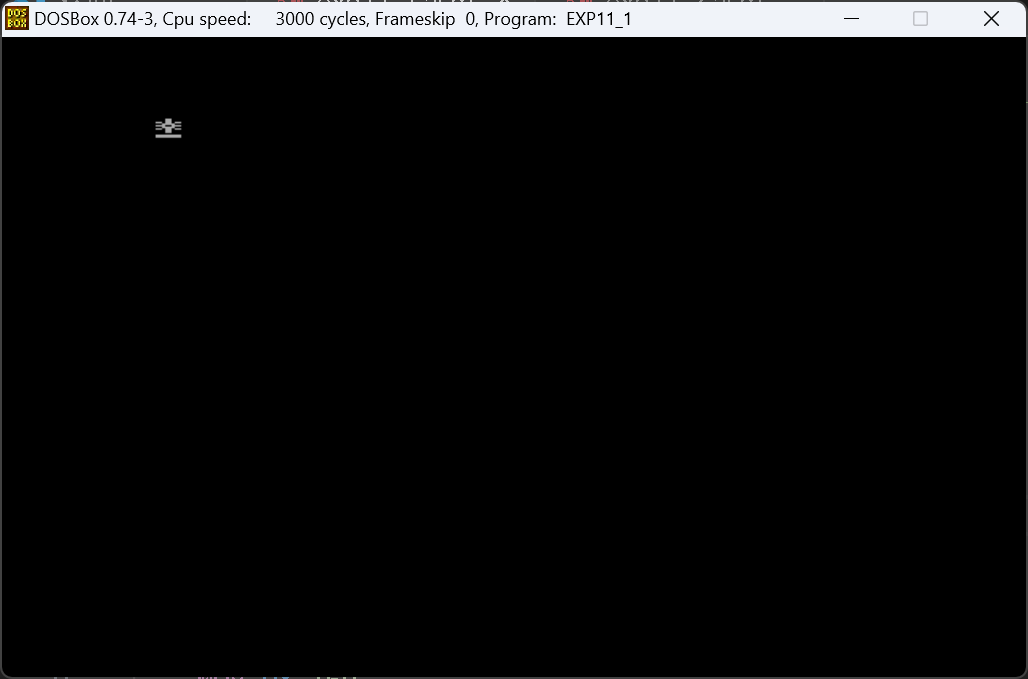
\includegraphics[scale=0.22]{pic/exp11-1-1.png}
    \caption{基础实验任务结果截图1}
    \label{基础实验结果截图1}
    \end{minipage}
    \hspace{0.05\textwidth}
    \begin{minipage}{0.45\textwidth}
    \centering
    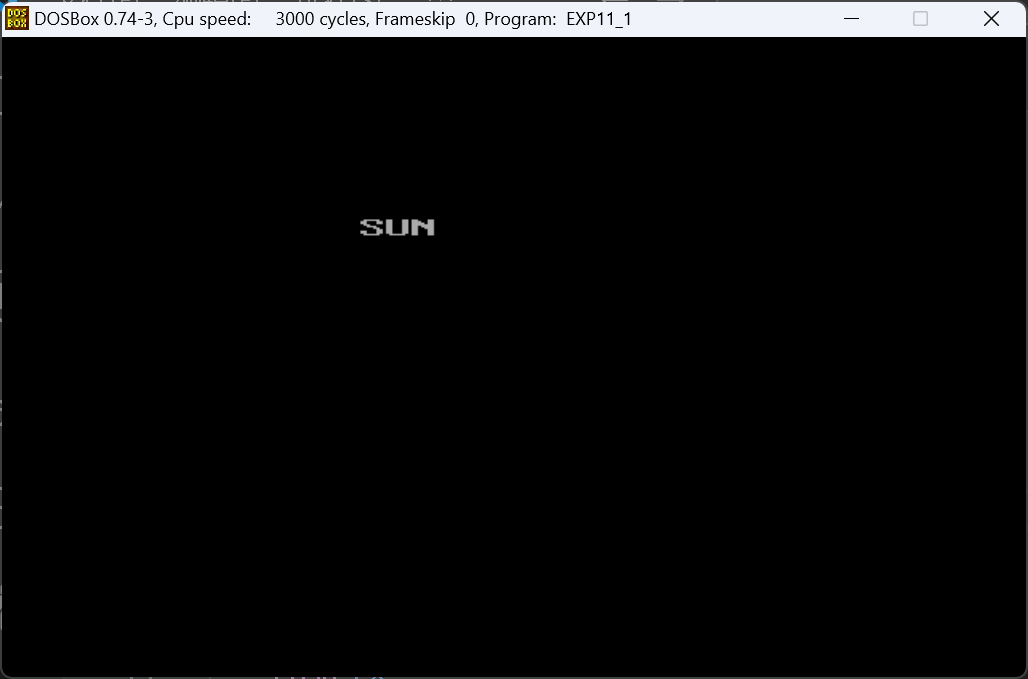
\includegraphics[scale=0.22]{pic/exp11-1-2.png}
    \caption{基础实验任务结果截图2}
    \label{基础实验结果截图2}
    \end{minipage}
\end{figure}
\begin{figure}[H]
    \centering
    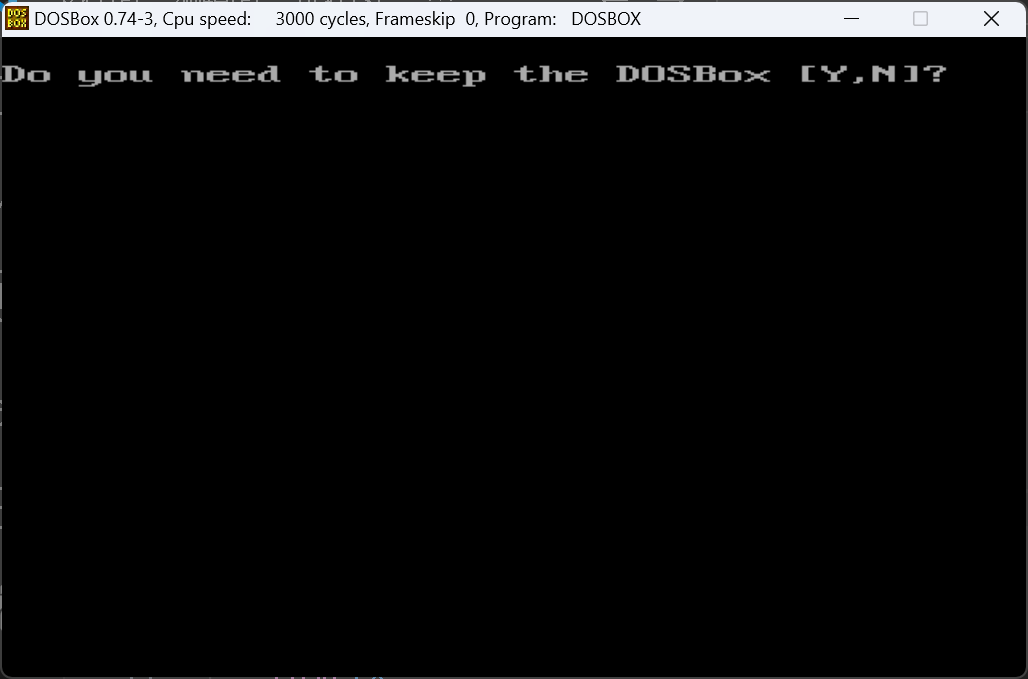
\includegraphics[scale=0.22]{pic/exp11-1-3.png}
    \caption{基础实验任务结果截图3}
    \label{基础实验结果截图3}
\end{figure}
\subsection{附加任务}
\subsubsection{实验任务的具体内容}
1)将累计定时中断次数改为设定一个定时的时间(如定时0.5秒、1秒、2秒……),每次定时时间到了就显示一次字符串1(显示字符串1的内容自己设置,希望同学们尽量不要雷同,字符串前面加上显示次数,后面加个空格);

2)定时显示12次字符串后,不等25行“太阳”图形显示完,就立即返回DOS;

3)在本次实验中加入实验十的键盘中断,在程序执行过程中,如果有按键,就显示一个字符串2(显示字符串2的内容也自己设置,尽量不要雷同,字符串前面加上按键次数,后面加个空格);如果定时时间到了就显示一次字符串1(字符串前面加上显示次数,后面加个空格)。 按键次数或定时显示次数只要有一个到12次了,就结束程序返回DOS;

注:按键先到12次和定时显示先到12次 这两种情况都要试一下。

4)将“太阳”图标和字符串改为彩色显示(彩色背景彩色字符),如,红底白字,蓝底黄字.

注:“太阳”图形、定时显示的字符串1和按键显示的字符串2最好用不同的颜色。
5)其他:鼓励同学们自己增加其他的附加功能。
\subsubsection{调试通过的源程序}
\begin{lstlisting}
    DATA SEGMENT
    TIMERTIME DB 00H
    SHOWTIMERTIME DB 00H,00H;SHOWTIMERTIME存放TIMERTIME对应的ASCII码
    STR1 DB 'TIMERINT!',20H
    N1 EQU $-SHOWTIMERTIME
    KEYTIME DB 00H
    SHOWKEYTIME DB 01H,00H;SHOWKEYTIME存放KEYTIME对应的ASCII码
    STR2 DB 'KEYINT!',20H
    N2 EQU $-SHOWKEYTIME
    COUNT1 DB N1
    COUNT2 DB N2
    TWELVE EQU 12;定义数值常量便于调试
    NUM EQU 36;一秒调用18.2次定时中断,据此计算
    ;定时0.5秒=9次,1s=18次,2秒=36次
    COUNTER DB NUM
DATA ENDS
CODE SEGMENT 
    ASSUME CS:CODE,DS:DATA
DELAY PROC         ; 延时程序
    PUSH CX
    PUSH DX
    MOV DX,36H
DL500:
    MOV CX, 08FFFH
DL10MS:
    LOOP DL10MS
    DEC DX
    JNZ DL500
    POP DX
    POP CX    
    RET
DELAY ENDP

DELAY2 PROC         ; 延时程序2
    PUSH CX
    PUSH DX
    MOV DX,1CH
DL5002:
    MOV CX, 01FFFH
DL10MS2:
    LOOP DL10MS2
    DEC DX
    JNZ DL5002
    POP DX
    POP CX    
    RET
DELAY2 ENDP

DISP1 PROC FAR     ; 显示太阳
    PUSH AX
    PUSH BX
    PUSH CX
    PUSH DX
    MOV AH,15     ; 读当前显示状态
    INT 10H
    MOV AL,1
    MOV AH,0      ; 设置显示方式
    INT 10H
    MOV DX,0      ; 行号为0,列号为0
REPT: 
    MOV AH,2      ; 设置光标位置
    INT 10H  
    MOV AL,0FH    ; OFH是太阳图形的ASCII码
    MOV CX,1      ; 重复字符的次数
    MOV BL,0F4H    ;字符颜色信息为橙底红字加闪烁(b7控制字符是否闪烁,b6-b4为背景色,b3-b0为前景色)
    MOV AH,9       ; 写字符
    INT 10H
    CALL DELAY
    SUB AL,AL
    MOV AH,0      ; 清除原图形
    INT 10H
    CMP KEYTIME,TWELVE;当键盘中断次数达到设定值时,直接结束显示
    JAE QUIT1 
    CMP TIMERTIME,TWELVE;当定时中断次数达到设定值时,直接结束显示
    JAE QUIT1 
    INC DH        ; 行号+1
    ADD DL,2      ; 列号+2
    CMP DH,20     ; 判断是否到20行,不等则继续显示太阳,相等返回
    JNE REPT
QUIT1:
    POP DX
    POP CX
    POP BX
    POP AX
    RET
DISP1 ENDP

INT_DISP1 PROC FAR    ; 定时中断显示信息
    PUSH DX
    PUSH CX
    PUSH BX
    PUSH AX
    PUSH SI
    MOV COUNT1,N1;用待显示的字符串的长度更新COUNT1
NEXTC: 
    LODSB  ; 字符串在数据段中定义并已经由SI指向首址
    MOV BH,00H
    MOV AH,03H
    INT 10H 
    MOV AH,9   ;写字符
    MOV CX,1      ;重复一次
    MOV BL,35H    ;字符颜色信息为青底紫字(b7控制字符是否闪烁,b6-b4为背景色,b3-b0为前景色)
    INT 10H
    INC DL ;每打印1个字符,光标的列号+1
    MOV AH,2      ; 更新光标位置
    INT 10H 
    CALL DELAY2 
    DEC COUNT1  
    CMP COUNT1,0 ;当整个中断信息串都显示完,才退出循环
    JA NEXTC
    POP SI
    POP AX
    POP BX
    POP CX
    POP DX
    RET
INT_DISP1 ENDP

INT_DISP2 PROC FAR    ; 键盘中断显示信息
; INT 10H 中AH=03H读取光标信息。入口参数:BH=显示页码
; 出口参数:CH=光标的起始行 CL=光标的终止行 DH=行(Y坐标) DL=列 (X坐标)
    PUSH DX
    PUSH CX
    PUSH BX
    PUSH AX
    PUSH SI
    MOV COUNT2,N2;用待显示的字符串的长度更新COUNT
NEXT: 
    LODSB  ; 字符串在数据段中定义并已经由SI指向首址
    MOV BH,00H
    MOV AH,03H
    INT 10H 
    MOV AH,9   ;写字符
    MOV CX,1      ;重复一次
    MOV BL,24H    ;字符颜色信息为绿底红字
    INT 10H
    INC DL ;每打印1个字符,光标的列号+1
    MOV AH,2      ; 更新光标位置
    INT 10H 
    CALL DELAY2 
    DEC COUNT2  
    CMP COUNT2,0 ;当整个中断信息串都显示完,才退出循环
    JA NEXT
    POP SI
    POP AX
    POP BX
    POP CX
    POP DX
    RET
INT_DISP2 ENDP

KEYINT PROC FAR 
    PUSH AX
    PUSH BX 
    PUSH DX 
    IN AL,60H      ; 通过8255A的PA口(PA口地址为60H)读取键盘扫描码
    MOV AH,AL
    IN AL,61H      ; 从8255APB口(PB口地址为61H)的PB7输出一个正脉冲(即PB7先输出高电平,再输出低电平)
    OR AL,80H      ; PB7置1
    OUT 61H,AL
    AND AL,7FH     ; PB7清零
    OUT 61H,AL     
    TEST AH,80H    ; 相等时代表键被释放,开中断,显示字符
    JNE BACK         
    STI  
    INC KEYTIME 
    MOV AX,0
    ADD AL,KEYTIME 
    AAA ;用于处理要显示的数字大于10的情况
    OR AX,3030H
    XCHG AL,AH
    MOV SI,OFFSET SHOWKEYTIME   ; 初始化SI,使其指向中断信息字符串首址
    MOV [SI],AX
    CLI 
    CALL INT_DISP2
    STI
BACK:
    MOV AL,20H
    OUT 20H,AL;结束中断
    POP DX
    POP BX
    POP AX
    IRET 
    KEYINT ENDP 

TIMERINT PROC FAR 
    PUSH AX		 ;保存寄存器
    PUSH BX
    PUSH CX
    PUSH DX
    PUSH DS    
    STI                  ;开中断
    DEC COUNTER
    CMP COUNTER,0
    JNZ QUIT ;不等于0,则直接退出;等于零,则:显示SUN,重置COUNTER,TIME+1
    MOV AX,NUM ;重置COUNTER
    MOV COUNTER,AX 
    INC TIMERTIME;TIMERTIME+1
    MOV AX,0
    ADD AL,TIMERTIME 
    AAA ;用于处理要显示的数字大于10的情况
    OR AX,3030H
    XCHG AL,AH
    MOV SI,OFFSET SHOWTIMERTIME   ; 初始化SI,使其指向中断信息字符串首址
    MOV [SI],AX
    CALL INT_DISP1
QUIT:
    CLI                  ;关中断
    POP	DS
	POP	DX
	POP	CX
	POP	BX
    POP	AX		      ;恢复寄存器  
    IRET	              ;中断返回
TIMERINT ENDP

START:
    MOV AX,DATA 
    MOV DS,AX 
    MOV AX,STACK
    MOV SS,AX
    MOV AX,0
    MOV ES,AX
    ; MOV SI,OFFSET TIME
    MOV AH,35H ;INT 21H 35H号:取中断向量,入口AL=中断类型,出口ES:BX=中断向量
    MOV AL,9
    INT 21H 
    PUSH BX ;将原键盘中断处理程序的CS:IP压栈
    PUSH ES 
    MOV AH,35H 
    MOV AL,1CH
    INT 21H 
    PUSH BX ;将原定时中断处理程序的CS:IP压栈
    PUSH ES
    MOV AX,0 ;恢复ES!重要!
    MOV ES,AX
    PUSH DS ;保护DS与DX!重要!
    PUSH DX
    CLI
    MOV AX,SEG KEYINT ;将自定义键盘中断服务程序的地址放入原09号中断向量处
    MOV DS,AX
    MOV DX,OFFSET KEYINT
    MOV AL,9
    MOV AH,25H ;INT 21H 25H号:设置中断向量,入口DS:DX=中断向量,AL=中断类型号
    INT 21H
    MOV AX,SEG TIMERINT ;将自定义定时中断服务程序的地址放入原1CH号中断向量处
    MOV DS,AX
    MOV DX,OFFSET TIMERINT
    MOV AL,1CH
    MOV AH,25H 
    INT 21H
    STI
    POP DX 
    POP DS 
AGIN:
    CALL DISP1
    CMP TIMERTIME,TWELVE
    JAE EXIT
    CMP KEYTIME,TWELVE
    JAE EXIT 
    JMP AGIN
EXIT:
    CLI               ; 禁止下方程序中断发生,保护代码运行
    POP DS  ;恢复原1CH号中断向量
    POP DX
    MOV AL,1CH
    MOV AH,25H
    INT 21H
    POP DS  ;恢复原09号中断向量
    POP DX
    MOV AL,9
    MOV AH,25H
    INT 21H
    STI               ; 开中断
    MOV AH,4CH
    INT 21H
CODE ENDS
END START 
\end{lstlisting}
\subsubsection{实验结果}
如图\ref{附加实验任务结果截图1}是程序正常运行的截图,太阳符号被修改为橙底红字加闪烁(附加功能4)。图\ref{附加实验任务结果截图2}是按一次键的运行截图。显示了绿底红字的中断信息"KEYINT!"并在该字符串前面显示了按键次数。图\ref{附加实验任务结果截图3}是定时中断服务程序的截图,显示了青底紫字的中断信息"TIMERINT!"并在该字符串前面显示了按键次数。图\ref{附加实验任务结果截图4}是第一种结束方式:定时显示先到12次,直接退出程序返回到DOS;图\ref{附加实验任务结果截图5}是第二种结束方式:按键先到12次。上述两种结束方式如图\ref{基础实验结果截图3}.完成附加功能1时,选择将定时设置为2秒,由于8253每隔55ms发一次定时中断请求信号,所以在定时中断服务程序中计数$2 \div 0.055 \approx 36$次后显示一次中断信息。
\begin{figure}[H]
    \centering
    \begin{minipage}{0.45\textwidth}
    \centering
    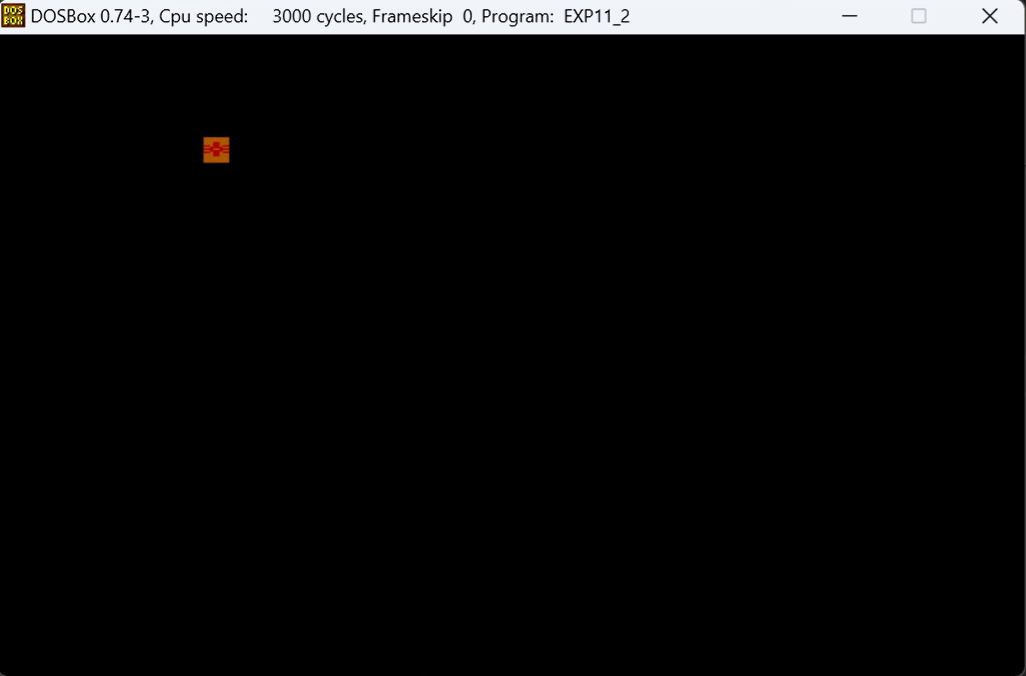
\includegraphics[scale=0.4]{pic/exp11-2-1.png}
    \caption{附加实验任务结果截图1}
    \label{附加实验任务结果截图1}
    \end{minipage}
    \hspace{0.05\textwidth}
    \begin{minipage}{0.45\textwidth}
    \centering
    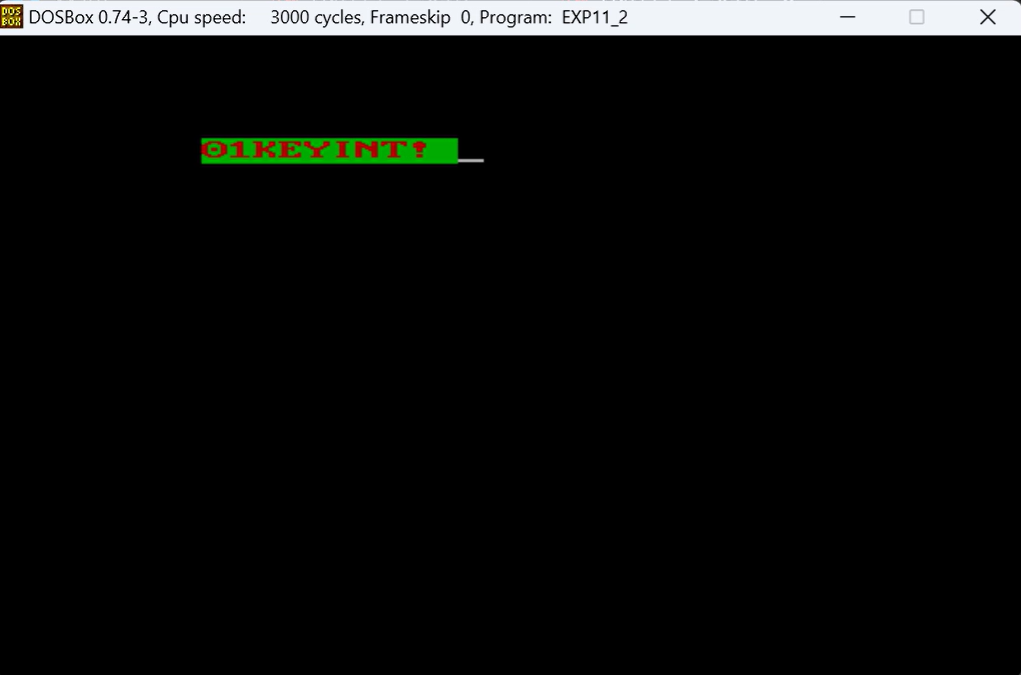
\includegraphics[scale=0.4]{pic/exp11-2-2.png}
    \caption{附加实验任务结果截图2}
    \label{附加实验任务结果截图2}
    \end{minipage}
\end{figure}
\begin{figure}[H]
    \centering
    \begin{minipage}{0.45\textwidth}
    \centering
    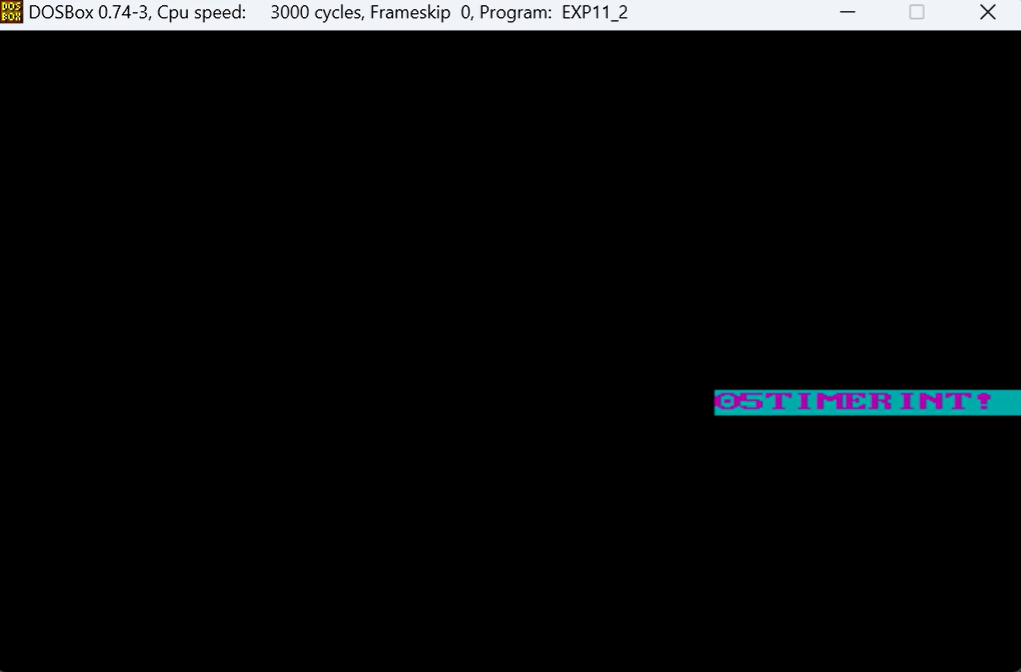
\includegraphics[scale=0.4]{pic/exp11-2-3.png}
    \caption{附加实验任务结果截图3}
    \label{附加实验任务结果截图3}
    \end{minipage}
    \hspace{0.05\textwidth}
    \begin{minipage}{0.45\textwidth}
    \centering
    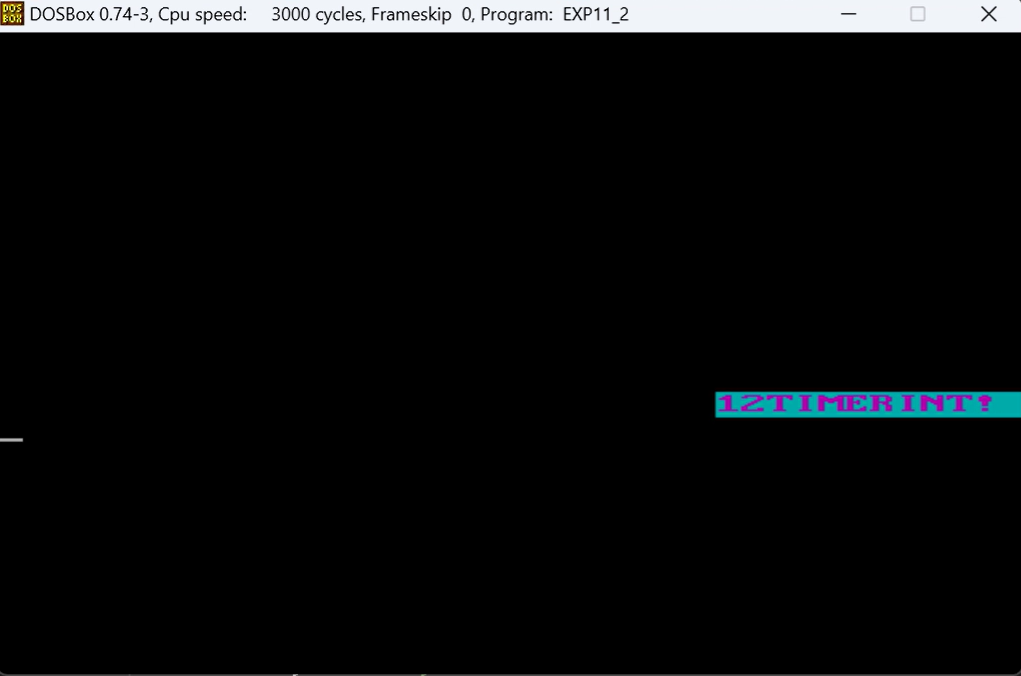
\includegraphics[scale=0.4]{pic/exp11-2-4.png}
    \caption{附加实验任务结果截图4}
    \label{附加实验任务结果截图4}
    \end{minipage}
\end{figure}
\begin{figure}[H]
    \centering
    \centering
    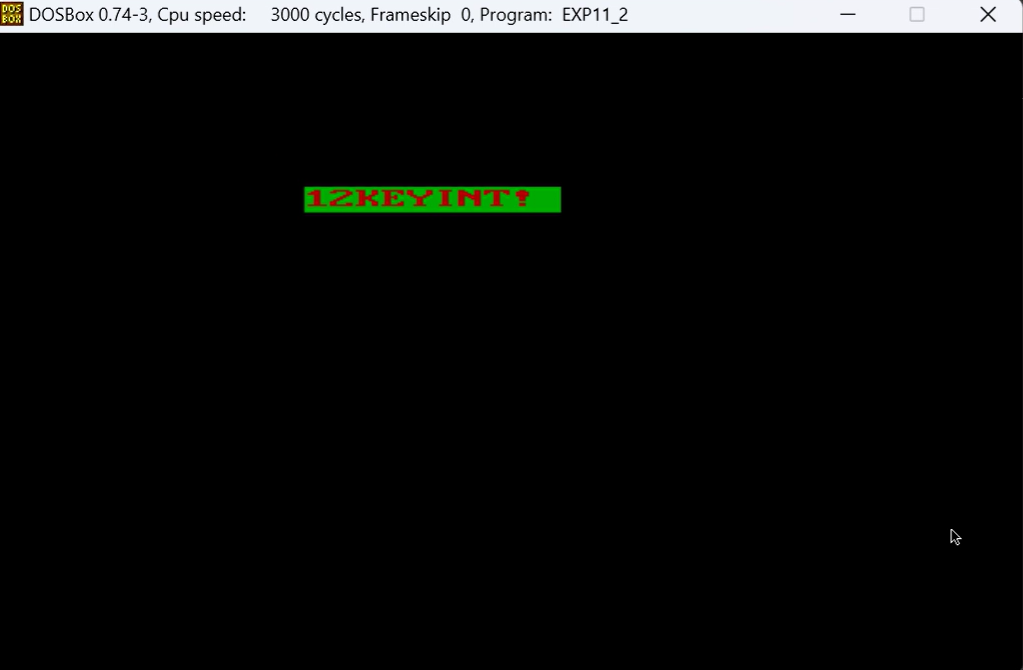
\includegraphics[scale=0.4]{pic/exp11-2-5.png}
    \caption{附加实验任务结果截图5}
    \label{附加实验任务结果截图5}
\end{figure}
\section{实验总结}
本次实验第二次涉及中断服务程序的设计。在设计过程中出现了以下问题:
\begin{enumerate}
    \item 每次太阳显示一轮之后就结束.错误原因:忘记在每次显示SUN之后将计数器TIME+1
    \item 定时中断显示信息从第二次开始输出乱码。错误原因:没有在每次输出后重置SI,没有将SI再次指向应打印的字符串首。
    \item 在第12次定时中断之后,太阳停留在左上角不动而没有返回DOS。错误原因:主程序跳转逻辑不对,应该是只要有任意一种中断显示达到12次就退出。
    \item 同一个段内的程序子段名不能一样,否则会跳转到错误的地方。
\end{enumerate}
\section{思考题}
% 1. 如果要求定时2秒左右显示一次字符串,那么,定时中断应该累计多少次显示一次字符串?
% 2. 完成附加功能的同学请回答:
% 1)在完成附加功能3)(加上实验十的键盘中断)时,如果程序运行结束返回DOS后,键盘不能正常使用,请分析一下可能会有哪些原因(至少写出三种原因)。
% 2)在完成附加功能3)时,如果在按键显示字符串2 时,各显示字符之间有延时,会遇到显示字符串2的字符中间会插入定时中断显示的字符串1的情况,请分析一下出现这种情况的原因,并说明如何修改程序才能避免这种情况。
\begin{enumerate}
    \item $2 \div 0.055 \approx 36$
    \item 原因1:中断向量未恢复,程序无法调用原始的键盘中断程序;原因2:编写子程序时没有保护用到的寄存器,某些寄存器的值被修改;原因3:硬件状态被非法修改,没有还原。
    \item 原因:在按键显示子程序运行过程中,定时中断进入,打断了正在运行的程序。解决办法:在编写自定义中断服务程序时手动关中断,禁止其他中断进入。
\end{enumerate}
\end{document}